%%%%%%%%%%%%%%%%%%%%%%%%%%%%%%%%%%%%%%%%%
% Stylish Article
% LaTeX Template
% Version 2.1 (1/10/15)
%
% This template has been downloaded from:
% http://www.LaTeXTemplates.com
%
% Original author:
% Mathias Legrand (legrand.mathias@gmail.com) 
% With extensive modifications by:
% Vel (vel@latextemplates.com)
%
% License:
% CC BY-NC-SA 3.0 (http://creativecommons.org/licenses/by-nc-sa/3.0/)
%
%%%%%%%%%%%%%%%%%%%%%%%%%%%%%%%%%%%%%%%%%

%----------------------------------------------------------------------------------------
%	PACKAGES AND OTHER DOCUMENT CONFIGURATIONS
\usepackage{placeins}
%----------------------------------------------------------------------------------------

\documentclass[fleqn,10pt]{SelfArx} % Document font size and equations flushed left

\usepackage[english]{babel} % Specify a different language here - english by default

\usepackage{lipsum} % Required to insert dummy text. To be removed otherwise

%----------------------------------------------------------------------------------------
%	COLUMNS
%----------------------------------------------------------------------------------------

\setlength{\columnsep}{0.55cm} % Distance between the two columns of text
\setlength{\fboxrule}{0.75pt} % Width of the border around the abstract

%----------------------------------------------------------------------------------------
%	COLORS
%----------------------------------------------------------------------------------------

\definecolor{color1}{RGB}{0,0,90} % Color of the article title and sections
\definecolor{color2}{RGB}{0,20,20} % Color of the boxes behind the abstract and headings

%----------------------------------------------------------------------------------------
%	HYPERLINKS
%----------------------------------------------------------------------------------------

\usepackage{hyperref} % Required for hyperlinks
\hypersetup{hidelinks,colorlinks,breaklinks=true,urlcolor=color2,citecolor=color1,linkcolor=color1,bookmarksopen=false,pdftitle={Title},pdfauthor={Author}}

%----------------------------------------------------------------------------------------
%	ARTICLE INFORMATION
%----------------------------------------------------------------------------------------

\JournalInfo{Text Mining \& Search Project} % Journal information
\Archive{A.Y. 2019-2020} % Additional notes (e.g. copyright, DOI, review/research article)

\PaperTitle{Methodological approaches for Text Summarization} % Article title

\Authors{\textbf{Riccardo Cervero}, \textbf{794126}\textsuperscript{1}} % Authors
\affiliation{\textsuperscript{1}\textit{Universita` degli Studi di Milano Bicocca, CdLM in Data Science}} 

\Keywords{Abstractive Summarization --- Extractive Summarization} % Keywords - if you don't want any simply remove all the text between the curly brackets
\newcommand{\keywordname}{Keywords} % Defines the keywords heading name

%----------------------------------------------------------------------------------------
%	ABSTRACT
%----------------------------------------------------------------------------------------

\Abstract{}

%----------------------------------------------------------------------------------------

\begin{document}

\flushbottom % Makes all text pages the same height

\maketitle % Print the title and abstract box

\tableofcontents % Print the contents section

\thispagestyle{empty} % Removes page numbering from the first page

%----------------------------------------------------------------------------------------
%	ARTICLE CONTENTS
%----------------------------------------------------------------------------------------

\section{Dataset} 
The texts to be summarized hails from a portion of the \href{https://www.kaggle.com/snap/amazon-fine-food-reviews}{"Fine Food Reviews"} dataset, recording 100,000 natural-language-written reviews in English from more than 70,000 Amazon users. The original data span from October 1999 up to October 2012, including, besides plain text reviews, product and user information, ratings and, above all, a very brew reference summary offered by database providers which will constitute the ground truth during the neural network training phase and an evaluation benchmark. As far as reviews, the average number of sentences is 5, while about one sentence on average is used to summarize the content. The number of sentences in the original document can affect extractive results of summarization, and its distribution shows, in the first case, a slight concentration around the mean\footnote{Reviews composed by a number of sentences between 3 and 7 are about 64\% of the total.}, with a very long and thin tail.
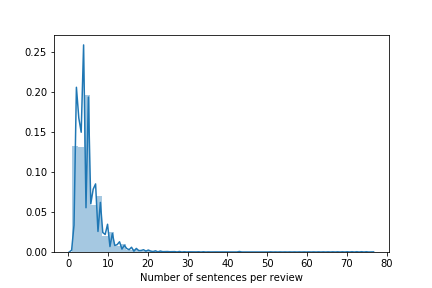
\includegraphics[width=9cm, height=5cm]{text_dist.png}
Nevertheless, even though this characteristic of homogeneity could help avoid bias during generation and comparison of several summaries, it is counterbalanced by a greater variability\footnote{While coefficient of variance for sentences count is about 74\%, the one related to word count is 102\%} in the number of words per review.
%------------------------------------------------
\section{Preprocessing}
Review is a particular kind of text, often composed by neither non-professional writer nor journalist which thus tends to resemble spoken language, because includes abbreviations, slang and informal phrases, errors in punctuation and misspellings, etc. This documents appear as a mixture of heterogeneous forms of text, even presenting different lexical and syntactic structures within the same document. For this reason, pre-processing operations are compulsory to help reduce distortion and try to convert the corpus into standard form.


%------------------------------------------------


\section{Extractive methods}

%------------------------------------------------

\section{Abstractive methods}

%------------------------------------------------

\section{Evaluation}
Only one sentence
%------------------------------------------------

\section{Results and Discussion}

%----------------------------------------------------------------------------------------
%	REFERENCE LIST
%----------------------------------------------------------------------------------------
\phantomsection
\bibliographystyle{unsrt}
\bibliography{sample}

%----------------------------------------------------------------------------------------

\end{document}
